\chapter{Traction machine case study}\label{chap:design}
In his last paper, \cite{Klima1979} wrote: ``The aim of designers of electrical machines is to design windings with winding factors for the working pole number as large as possible and at the same time to suppress the rest of the winding factors''. This design strategy is still valid today. 

This chapter is devoted to the main research question. In the first half up to section \ref{sec:prototype} a fast and accurate design procedure is developed which is suitable for an everyday design environment. For the case study, the procedure presented is  applied to a \SI{150}{kW} traction machine with a single layer non-overlapping windings and interior permanent magnets. The design is aimed at integrated drives for the use in underground and city trains as presented by \cite{Joeckel2006}. From section \ref{sec:prototype} the measured results of the realised prototype are offered and discussed. 

\section{Introductory remarks}
The design of high-performance machine drives requires a detailed understanding of machine characteristics and associated interactions with power electronic devices.  Although the basic principle of operation for a given machine type stays the same, the detailed design is defined by the application and the environmental conditions. These can be very different for low and high power drives.

When designing electrical machines the primary aim is to find the major dimensions which are the bore diameter and the stack length. Usually the final design is found through an iterative optimisation process that is applied to the initial design parameters. The two most important electromagnetic requirements are the magnetic and electrical loading. All design parameters are then expressed in terms of the flux and current densities for which there are some guideline values. Very seldom a machine design is started from scratch and it is typical to use an available machine and adapt it to the design requirements.

The requirements of the electromagnetic design is specified by the torque versus speed characteristic for the driving and braking mode. This describes the machine behaviour over the whole speed range. It is the aim of the designer to find the best geometrical dimensions that fulfil the torque versus speed characteristic. The optimisation criteria depend on the application. For trains that are operated in the city, where they have to accelerate after each stop, the objective would be to keep the average loss over a cycle to a minimum. In high speed applications, the traveling time between two stops is much longer than those for city trains. Here the objective would be to optimise the efficiency at the speed where the motors are operated most of the time. 

%\section{Torque versus speed characteristic}
%The traction drive under consideration is designed for a low voltage d.c.~grid with a nominal d.c.~voltage of \SI{750}{V} on third rail. A typical design starts with a torque versus speed characteristic and for traction applications it needs to be specified for both the driving and braking mode. The maximum values of the drive specification are given in Tab.~\ref{tab:DriveSpecification} and the characteristics for braking and driving are given in Fig.~\ref{fig:torq_speed}(a) and (b) respectively. The given power characteristics are only short time values during the acceleration or braking phase, which is typically between \SI{10}{s} and \SI{20}{s}. Consequently, the required power is not a thermal rating. The two operating modes can be summerised as follows:
%\begin{description}
  %\item[Braking:] Characteristic for the braking mode is the relatively long constant~%
  %torque region and the short constant power range. In braking mode the machine is~%
  %operated as a generator, supplying power to the grid. During braking mode the vehicle~%
  %can easily deal with double the traction power. The additional power is used to~%
  %supply auxiliaries and other vehicles with the braking power. Excess power can easily~%
  %(if necessary) be dissipated through a d.c.~dump resistor. For this reason the~%
  %d.c.-bus~%
  %voltage is higher than in driving mode. From the train operator the d.c.-bus voltage~%
  %during braking is specified as \SI{900}{V}. This means that the output line-to-line~%
  %voltage of the~%
  %inverter in braking mode is higher than in the case of driving mode. Moreover, the~%
  %number of series turns must be chosen in such a way as to ensure that the pullout~%
  %torque is at least \SI{10}{\%}-\SI{15}{\%} higher than the torque at maximum speed~%
  %during braking. 
  %\item[Driving:] In this mode the machine is operated as a motor. The available power~%
  %in driving mode is limited by the d.c.~supply grid. The machine is~%
  %operated most of the operating time in this mode. Therefore, the objective is to~%
  %find the best geometrical dimensions that ensure the maximum torque per~%
  %current. Since the braking mode is used to determine the number of series turns,~%
  %it often occurs that the maximum line-to-line voltage is reached in the constant~%
  %power region (and not at the beginning of the constant power region). From this~%
  %point on up to the maximum speed, field weakening is required. From the train~%
  %operator the d.c.-bus voltage is specified as \SI{730}{V}.  
%\end{description}
%\begin{table}[htbp]
  %\centering
  %\caption{Drive specification (maximum values)}
    %\begin{tabular}{|l|c|c|}\cline{2-3}
      %\multicolumn{1}{c|}{}& Braking (Generator) & Driving (Motor) \\
      %\hline
      %$P_{mech}/\SI{}{kW}$ & 300 & 150 \\
      %$U_{d.c.}/\SI{}{V}$  & 900 & 750 \\
      %$U_{1,max}/\SI{}{V}$ & 702 & 585 \\
      %$n_{max}/\SI{}{rpm}$ & 700 & 700 \\
      %\hline
    %\end{tabular}
  %\label{tab:DriveSpecification}
%\end{table}
%\begin{figure}[htbp]
  %\centering
    %\input{figs/ch5/f_Mn.tex}
  %\caption{Traction machine torque speed characteristic}
  %\label{fig:torq_speed}
%\end{figure}

\section{Conceptional design}
The conceptional design starts with the choice of the main geometrical dimensions. In this step the volume that encloses the air gap is determined. The air gap volume is obtained from the bore diameter and effective stack length. Guideline values for current density can be used to obtain all the design parameters to be optimised. 
If there are no further requirements, these parameters are then fine-tuned by means of an iterative process in order to get the best solution to fit the given design requirement.    
Often requirements like cost reduction lead to designs that are optimised for the manufacturing process. In such a case non-overlapping windings are definitely very attractive, especially due to the simple construction. 

\subsection{Winding type}
In applications where machines are operated with an inverter supply the induced turn-to-turn voltages could be twice the normal operating voltage. For contaminant-laden environments the end windings are the most susceptible area. Moisture and contaminants increase tracking and deterioration that can lead to failure. Aspects like these limit the choice of wire and the type of insulation. The wire type and insulation not only determine the copper fill factor, but the loss calculation as well.

\subsubsection{Form-wound versus random-wound coils}
Fig.~\ref{fig:insulation} shows typical winding configurations that could be used in the design. The choice of winding configuration does not affect the electromagnetic behaviour of the machine, but it does affect the loss mechanism. Form-wound coils have a much better copper fill factor. This means that for the same current it will have a lower resistance compared to its round-wire counterpart and consequently lower copper loss.   
\begin{figure}[htbp]
  \centering
  \subfloat[Single layer]{
  \begin{psfrags}%
\psfragscanon

% text strings:
\psfrag{t01}[bc]{{\tiny Round wire}}
\psfrag{t02}[bc]{{\tiny Form wound coils}}
\psfrag{t03}[bc]{{\tiny Single layer}}
\psfrag{t04}[bc]{{\tiny Double layer}}
\psfrag{t05}[bc]{{\tiny Single layer}}
\psfrag{t06}[bc]{{\tiny Double layer}}
\psfrag{t07}{{\tiny $h_1$}}
\psfrag{t08}{{\tiny $h_1$}}

% Figure:
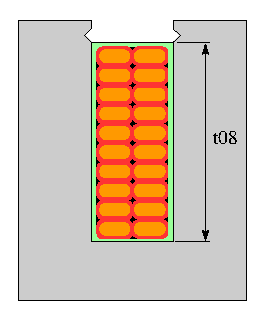
\includegraphics[width=0.21\textwidth]{figs/f_insulation_c.eps}
\end{psfrags}%}
  \hfill
  \subfloat[Double layer]{
  \begin{psfrags}%
\psfragscanon

% text strings:
\psfrag{t01}[bc]{{\tiny Round wire}}
\psfrag{t02}[bc]{{\tiny Form wound coils}}
\psfrag{t03}[bc]{{\tiny Single layer}}
\psfrag{t04}[bc]{{\tiny Double layer}}
\psfrag{t05}[bc]{{\tiny Single layer}}
\psfrag{t06}[bc]{{\tiny Double layer}}
\psfrag{t07}{{\tiny $h_1$}}
\psfrag{t08}{{\tiny $h_1$}}

% Figure:
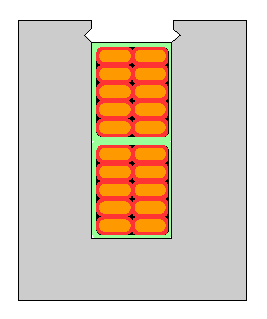
\includegraphics[width=0.21\textwidth]{figs/f_insulation_d.eps}
\end{psfrags}%}
  \hfill
  \subfloat[Single layer]{
  \begin{psfrags}%
\psfragscanon

% text strings:
\psfrag{t01}[bc]{{\tiny Round wire}}
\psfrag{t02}[bc]{{\tiny Form wound coils}}
\psfrag{t03}[bc]{{\tiny Single layer}}
\psfrag{t04}[bc]{{\tiny Double layer}}
\psfrag{t05}[bc]{{\tiny Single layer}}
\psfrag{t06}[bc]{{\tiny Double layer}}
\psfrag{t07}{{\tiny $h_1$}}
\psfrag{t08}{{\tiny $h_1$}}

% Figure:
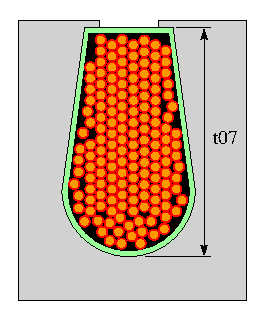
\includegraphics[width=0.21\textwidth]{figs/f_insulation_a.eps}
\end{psfrags}%}
  \hfill
  \subfloat[Double layer]{
  \begin{psfrags}%
\psfragscanon

% text strings:
\psfrag{t01}[bc]{{\tiny Round wire}}
\psfrag{t02}[bc]{{\tiny Form wound coils}}
\psfrag{t03}[bc]{{\tiny Single layer}}
\psfrag{t04}[bc]{{\tiny Double layer}}
\psfrag{t05}[bc]{{\tiny Single layer}}
\psfrag{t06}[bc]{{\tiny Double layer}}
\psfrag{t07}{{\tiny $h_1$}}
\psfrag{t08}{{\tiny $h_1$}}

% Figure:
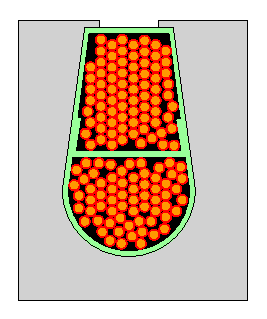
\includegraphics[width=0.21\textwidth]{figs/f_insulation_b.eps}
\end{psfrags}%}
  \caption{Typical form-wound and random-wound coils} 
  \label{fig:insulation}
\end{figure}
A summary of the main differences between form-wound and random-wound coils are given in Tab.~\ref{tab:form_vs_round}
\begin{table}
\caption{Main differences between form- and random-wound coils}
\label{tab:form_vs_round}
\begin{tabularx}{\textwidth}{XX}
\toprule
\textbf{Form-wound coils}  & \textbf{Random-wound coils} \\\toprule
The magnet wire is rectangular or square and individual turns are systematically arranged throughout the coil. & 
Round-wire of equal or different sizes is used and the turns have a random location.\\\midrule
Individual wires are held tightly in the slot and the copper fill is uniform. &
The individual wires may be loose and vibrate with respect to each other, depending on the resin treatment.\\\midrule
Coil-to-coil connections are usually required. &
Only phase connections are required. \\\midrule
All the coils have an identical end winding form which mean that there are large openings for air circulation. This prevents contamination build up. In addition the large openings promote cooling.&
End windings are completely covered and excessive resin can build up. The openings are usually sealed which means that moisture and contaminates can easily be accumulated.  
\\\bottomrule
\end{tabularx}
\end{table}

\subsubsection{Single versus double layer non-overlapping windings}
Since the analysis in the present dissertation is devoted to non-overlapping windings, the choice should be made between single and double layer. A summary of the differences are given in Tab.~\ref{tab:single_vs_double_2}.
\begin{table}[htbp]
\caption{Summary of single and double layer winding coils}
\begin{tabularx}{\textwidth}{XX}
\toprule
\textbf{Non-overlapping double layer}&\textbf{Non-overlapping single layer}\\\toprule 
A non-overlapping double layer concentrated winding has a coil wound around each tooth and the coil pitch is fixed.  This usually leads to the use of round-wire for which the insulation class \num{200} is not typical. The number of coils is equal to the number of slots. To reduce the cogging torque any further the rotor must be skewed. &
Here only every second stator tooth has a coil wound around it and as a consequence the coil pitch can be varied to improve the motor performance. This then leads to a stator design with alternating tooth widths. Form-wound coils and insulation class \num{200} can be used and the coil number is half the slot number. It is not necessary to skew the rotor since the stator slot pitch can be varied to reduce the cogging torque.
\\\bottomrule
\end{tabularx}
\label{tab:single_vs_double_2}
\end{table}

Due to environmental conditions, it is typical to use form-wound coils in traction machines rather than random-wound coils\footnote{Also known as round-wire.}. Form-wound coils have a better thermal loading and vibration withstand capability. 

%\subsection{Sizing equations}
%A general sizing equation that can be used to find the main dimensions is the so-called Esson number. It is defined as the torque corresponding to the apparent power $P_s$ to the air gap bore volume. \cite{Gutt1998} summarized the Esson number in their paper as
%\begin{equation}
  %\label{eqn:Esson}
  %C = \frac{P_s}{2\pi n V_{bore}}=\frac{\pi^2}{\sqrt{2}}\xi_p A_1 \hat{B}_{\delta}
  %\quad
  %\begin{cases}
    %A_1 = 2m\cfrac{N_s I_1}{\pi d_{i1}} \\
    %\: \\
    %\hat{B}_{\delta} = \cfrac{2p\hat{\Phi}}{2ld_{i1}}\\
    %\: \\
    %V_{bore}=\cfrac{\pi d_{i1}^{2}}{4}l_{Fe}
  %\end{cases}  
%\end{equation} 
%and pointed out that the equation parameters cannot be applied to linear machines. \cite{Ronghai2004} used the same argument and suggested a method that is valid for all machine types. This of course is only useful if different machine types are to be compared with each other. Since their is no exact design rule to calculate the machine parameters, the Esson number is a good starting point. The reader is referred to the book of \cite{Vogt1996} for detailed lists of typical $A_1$ and $B_{\delta}$ for different machine types. 
%
%\subsection{Number of stator slots}\label{subsec:number_of_slots}
%The specifications for the stator slots are that they must be open, since form-wound stator coils must be used. The case study prototype motor presented in the present dissertation has a stator inner diameter of \SI{280}{mm} (a detailed drive specification was presented by \cite{germishuizen_2006} and \cite{joeckel_2006}). Choosing the number of stator slots is bounded by primarily two factors:
%\begin{enumerate}
  %\item For single layer non-overlapping windings the number of stator slots must~%
  %be a multiple of twice the number of phases, i.e.~%
  %$Q_{s} \in \left\{6,12,18,24,\ldots\right\}$.
  %\item Design for manufacturability means that products are designed in such a~%
  %way that they are easy to manufacture at the lowest possible cost.
%\end{enumerate}
%
%For the stator inner diameter of \SI{280}{mm} the possible slot number is in the range  $24 \leq Q_s \leq 36$. Tab.~\ref{tab:wnd_char} gives the properties of the winding for the different slot and pole pair combinations. Since non-overlapping concentrated form-wound stator coils are used to achieve a high copper fill factor, the tooth width around which the coils are wound limits the radius of curvature. For manufacturing, the best number of slots is chosen to be $Q_{s}=30$. It was shown in section \ref{subsec:wind_fac_table} that the feasible region for the number of slots per pole and phase should be $\frac{1}{4} \leq q \leq \frac{1}{2}$. \cite{skaar_2006} presented the same results in their conference paper. For manufacturability the least number of poles are chosen, i.e.~for $q=\frac{1}{2}$. Therefore the number of pole pairs equals  $p=10$. For this design the average coil pitch is $y_p = 1.5$, and since it is a single layer non-overlapping winding $y_d=1$. For analysis purposes it is necessary to keep track of both the average coil pitch and the actual chosen coil pitch.
%\begin{table}[htbp]
  %\centering
  %\caption{Slot and pole pair combinations for case study design}
  %\begin{tabular}{p{1.2cm}p{1.2cm}p{1.2cm}p{1.2cm}p{1.2cm}p{1.2cm}p{1.2cm}}
  %\toprule
  %$Q_s  $    &   24  &  24  & 30 & 30 & 36 & 36 \\\midrule
  %$p    $    &   8   &  10  & 10 & 13 & 12 & 15 \\\midrule
  %$Q_c  $    &   12  &  12  & 15 & 15 & 18 & 18 \\\midrule
  %$q    $    &$\frac{1}{2}$&
              %$\frac{2}{5}$&
              %$\frac{1}{2}$&
              %$\frac{5}{13}$&
              %$\frac{1}{2}$&
              %$\frac{2}{5}$\\\midrule
  %$q_{c}$    &$\frac{1}{4}$&
              %$\frac{1}{5}$&
              %$\frac{1}{4}$&
              %$\frac{5}{26}$&
              %$\frac{1}{4}$&
              %$\frac{1}{5}$\\\midrule
  %$Q_b$      &  6   &  12  &  6  & 30 & 6 & 18 \\\midrule
  %$t$        &  4   &  2   &  5  & 1  & 6 & 3  \\\midrule
  %$\xi_p$    & 0.866 & 0.966 & 0.866 & 0.936 & 0.866 & 0.966 \\\bottomrule
  %\end{tabular}
  %\label{tab:wnd_char}
%\end{table}
%
%\subsection{Electromagnetic design}
%The geometrical dimensions of the electromagnetic design are limited by the available space. In railway traction, as in this example, the available space is limited by the gauge, which is standard gauge\footnote{Also named the Stephenson gauge after George Stephenson.}. The distance between the inside edges of the rails of a standard gauge track is \SI{1435}{mm}. In addition to this, the diameter of the wheels and the required  underground clearance determine the maximum stator outer diameter. Another requirement that limits the design is the specification to use insulation class \num{200}. Usually this leads to the use of form-wound coils. The electromagnetic design and its parameters are shown in Fig.~\ref{fig:FEA_design}.
%\begin{figure}[htbp]
  %\centering
    %\input{figs/ch5/f_fea_design.tex}
  %\caption{Geometrical machine parameters}
  %\label{fig:FEA_design}
%\end{figure}
%
%\subsection{Winding properties}
%The use of form-wound coils means that the inner slot walls of the tooth around which the oil is wound, could be parallel to each other. One advantage thereof is that it is very easy to insert the coils into the stator slots. The major winding properties are presented in this section. 
%
%\subsubsection{Effective number of turns per slot}
%In practical engineering these variables are expressed in terms of the winding parameters and the arrangement of the conductors in the stator slot. The effective number of turns is 
%\begin{equation}
  %\label{eqn:z}
  %z = \frac{m_{sl}n_{sl}}{a_w a}
  %\quad
  %\begin{cases}
  %m_{sl} & \mbox{wires in slot height} \\
  %n_{sl} & \mbox{wires in slot width}  \\
  %a_w    & \mbox{parallel wires} \\
  %a      & \mbox{parallel branches} \\
  %\end{cases}
%\end{equation} 
%
%\subsubsection{Series number of turns}
%For the calculation of the induced voltage per phase, only the number of series turns is necessary. The number of series turns is calculated as
%\begin{equation}
  %\label{eqn:Ns}
  %N_s = z\frac{Q_s}{2m}
%\end{equation}
%where $z$ is the effective number of turns per slot as given in \eqref{eqn:z}.
%
%\subsubsection{End winding leakage inductance}\label{sec:Le}
%Fig.~\ref{fig:wend_winding}(a) shows a cross section of the machine and the location of the end winding. Although the leakage inductance is usually difficult to calculate analytically and must be determined by approximate or empirical techniques, it plays an important role in machine performance. The end winding leakage inductance is calculated as
%\begin{equation}
  %\label{eqn:Lsigma}
  %L_e = \mu_0 l_e q z^{2} \frac{Q_s}{m} \lambda_e
%\end{equation}
%where $\lambda_e$ is the specific permeance of the end winding and $l_e$ is the average length of the end winding. Using the parameters in Fig.~\ref{fig:wend_winding}(b), $l_e$ is calculated as
%\begin{equation}
  %\label{eqn:le}
  %l_e = \pi\frac{b_t+b_s}{2}+2l_{se}
%\end{equation} 
%where $l_{se}$ is the straight part of the winding overhang. Due to the mechanical construction, it is difficult to calculate the specific permeance of the end winding and it is therefore estimated on the basis of experiments.  \cite{Gieras2002} mention in their book that 
%\begin{equation}
  %\lambda_e \approx 0.2q
%\end{equation}  
%gives good results for single layer windings. 
%\begin{figure}
  %\centering
    %\input{figs/ch5/f_end_winding.tex}
  %\caption{End winding parameters}
  %\label{fig:wend_winding}
%\end{figure}
%
%\subsubsection{Stator d.c.~winding resistance}
%The stator winding resistance per phase for the d.c.~current is 
%\begin{equation}
  %\label{eqn:R1a}
  %R_1 =  \frac{zQ_s}{m} \frac{l_{av}}{\sigma A_{cu}}
%\end{equation}
%where $l_{av}$ is the average length of a turn, $A_{cu}$ is the wire cross section and $\sigma$ the conductivity at given temperature (for copper~%
%$\sigma = \SI{57.14e6}{S.m^{-1}}$ at \SI{20}{\degC}. The average length of a winding turn is calculated as
%\begin{equation}
  %\label{eqn:lav}
  %l_{av} = 2(l_{Fe}+l_e)
%\end{equation} 
%in which $l_{Fe}$ is the stack length (the machine has no radial cooling ducts) and $l_e$ is given in \eqref{eqn:le}. Usually the resistance is calculated for \SI{20}{\degC}. Under operating conditions the temperature coefficient of copper $\alpha$ is used to calculated the resistance at a temperature $T_c$ as
%\begin{equation}
  %R = R_{1,\SI{20}{\degC}}(1+\alpha \Delta T)
  %\quad
  %\begin{cases}
  %\alpha = 0.00395\\
  %\Delta T = T_c-\SI{20}{\degC}
  %\end{cases}
%\end{equation} 
%
%\subsubsection{Winding layout}
%The winding layout is obtained directly from the winding matrix. Fig.~\ref{fig:w_layout} shows the final winding layout. Since the basic winding has 6 slots and 3 coils, the basic winding is repeated 5 times. Recall from chapter \ref{chap:DesignWindings} that the winding matrix of the basic winding equals 
%\begin{equation}
  %\mathbf{M_{1,b}} = 
  %\begin{pmatrix}
  %1&0&0&0&0&0\\
  %0&0&1&0&0&0\\
  %0&0&0&0&1&0\\
  %\end{pmatrix} \
  %\mathbf{M_{2,b}} = 
  %\begin{pmatrix}
  %0&-1&0&0 &0&0 \\
  %0&0 &0&-1&0&0 \\
  %0&0 &0&0 &0&-1\\
  %\end{pmatrix} 
%\end{equation}
%and $\mathbf{M_{1,b}}(1,1)=1$, it means that the ingoing coil side of phase 1 of the first is positive. The outgoing coil side is negative and $\mathbf{M_{2,b}}(1,2)=-1$. 
%\begin{figure}[htbp]
  %\centering
    %\input{figs/ch5/f_layout.tex}
  %\caption{Winding layout}
  %\label{fig:w_layout}
%\end{figure}
%
%\subsection{Geometrical dimensioning}
%Through an iterative design procedure the geometrical dimensions need to be determined. The focus in this section is to show how the variable pitch of single layer non-overlapping windings can be used to improve the design. 
%
%\subsubsection{No-load flux linkage versus tooth width}
%From the winding design methods presented in chapter \ref{chap:DesignWindings}, the single layer non-overlapping winding type can have a variable coil pitch. To illustrate the influence of changing the coil pitch as defined in \eqref{eqn:slot_alpha} the value of $x$ is varied between \num{1} and \num{1.5}. For $x=1$ it is a regular distribution of the stator slots as shown in Fig.~\ref{fig:f_slotstar}(a). If $x>1$, the slots have a irregular distribution as shown in Fig.~\ref{fig:f_slotstar}(b). The winding factors for different values of $x$ and $p$ are given in Tab.~\ref{tab_factors}. Setting $x=1$ the winding factor equals \num{0.866}. This is the same as reported by \cite{cros_2002}; \cite{IR-EE-EME_2003:029}; \cite{skaar_2006}; and \cite{libert_2004}. If $x=y_{p}$ it means that the coil spans a pole pitch and the winding factor equals 1.
%\begin{table}[htbp]
  %\centering
  %\caption{Winding factors when changing the slot pitch ($x\tau_s$)}
  %\begin{tabular}{l@{\hspace{10mm}}%
                  %l@{\hspace{10mm}}%
                  %l@{\hspace{10mm}}%
                  %l@{\hspace{10mm}}%
                  %l}
      %\hline
      %$x$  & $\xi_{5}$ & $\xi_{10}$ & $\xi_{50}$ & $\xi_{70}$   \\
      %\hline
      %1.00 & 0.50      & 0.87       & 0.87       & 0.87         \\
      %1.05 & 0.52      & 0.89       & 0.71       & 0.99         \\
      %1.10 & 0.54      & 0.91       & 0.50       & 0.98         \\
      %1.15 & 0.57      & 0.93       & 0.25       & 0.83         \\
      %1.20 & 0.59      & 0.95       & 0.00       & 0.59         \\
      %1.25 & 0.61      & 0.96       & 0.26       & 0.26         \\
      %1.30 & 0.63      & 0.97       & 0.50       & 0.10         \\
      %1.50 & 0.71      & 1.00       & 1.00       & 1.00         \\
     %\hline   
  %\end{tabular}
  %\label{tab_factors}
%\end{table}
%
%The results presented in Tab.~\ref{tab_factors} means that the winding factor will become a function of the tooth width. Since the induced voltage is directly proportional to the winding factor as given in \eqref{eqn:ui}, the flux linkage $\xi_p N_s \hat{\Phi}$ will also be a function of the tooth width ($b_t$ in \ref{fig:FEA_design}). The winding factor calculation is verified by means of FEA. Instead of calculating the air gap field harmonics, the flux linkages when moving the rotor is evaluated for a given magnet and slot width. The FEMP software employs a special air gap element in the finite element method as proposed by \cite{razek_1981}, is used (a summary of the air gap element is given in appendix \ref{app:AGE}). There is no mesh in the air gap, which means that the rotor rotation is independent of the mesh and a suitable step size can be chosen that will simplify the discrete Fourier transformation of the flux linkages. Fig.~\ref{fig:fieldsol} shows a field solution of the FEMP software\footnote{Only a limited version for displaying the FEM calculated results, was programed in Matlab.}. Notice that there is no mesh in the air gap.  
%\begin{figure}[htbp]
  %\centering
    %\includegraphics[width=0.70\textwidth]{figs/ch5/f_vec.eps}
    %\caption{No-load field solution using FEMP}
  %\label{fig:fieldsol}
%\end{figure}
%
%The result of the fundamental flux linkage for different tooth widths is shown in Fig.~\ref{fig:Main_bt_design}\subref{fig:psi_bt}. This verifies that by increasing the tooth width, the fundamental winding factor can be increased.
%
%\subsubsection{Torque pulsation}\label{subsubsec:torque_pulsations}
%There are three sources of torque ripple coming from the machine. They are: the cogging effect; distortion of the magnetic flux density distribution in the air gap; and the difference between permeances of the air gap in the $d$- and $q$-axis. Cogging torque in permanent magnet machines is caused by the interaction between the rotor magnetic flux and the variable permeance of the air gap due to the stator slot geometry. For regular distributed stator slots the number of cogging pulsations per rotor revolution is a function of the least common multiple between $Q_{s}$ and $2p$ as mentioned by \cite{cros_2002}, i.e.~$\textnormal{lcm}\left(Q_{s},2p\right)$ and should be as high as possible.
%\begin{figure}[htbp]
  %\centering
  %\input{figs/ch5/f_psi_bt.tex}
  %\input{figs/ch5/f_T_ripple.tex}
  %\caption{Tooth width as design parameter}
  %\label{fig:Main_bt_design}
%\end{figure}
%
%Once the stator slot parameters are chosen, the stator tooth width is varied to minimise the cogging torque. The torque as a function of the rotor position is calculated from the AGE and by rotating the rotor in the FE analysis. Fig.~\ref{fig:Main_bt_design}\subref{fig:T_ripple} shows the torque harmonics as a percentage of the rated torque. It can be seen that the $6^{th}$ torque harmonic can be reduced to zero if the tooth width is chosen to be $\SI{26.6}{mm} \leq b_t \leq \SI{26.9}{mm}$. The irregular distribution of the stator slots has another advantage which reduces the no-load cogging torque.
%
%\subsubsection{Rotor design}
%In the electromagnetic design of the rotor the main objective is to find the magnet dimensions. It should be chosen in such as way that the interactions of the rotor air gap mmf harmonics with that of the stator winding are minimized. In order to do so, the working harmonic of the rotor air gap mmf needs to be evaluated. Fig.~\ref{fig:Main_f_dft_id0} showed the air gap mmf harmonics with zero current and a regular distribution of the stator slots. In this case the air gap mmf have both a $5^{th}$ and $7^{th}$ spatial harmonic. Fig.~\ref{fig:mag_entwurf} shows the spatial harmonics of the air gap mmf. The magnet width is chosen such that the $5^{th}$ and $7^{th}$ spatial harmonics are suppressed. In doing so, however, a sub-harmonics arises.
%
%The mechanical design of the rotor comprises, among others, two mechanical parameters. They are the bridge height $h_b$ and the web width $b_w$ as shown in Fig.~\ref{fig:FEA_design}. The laminated bridge above the magnets and closest to the air gap has its minimum height between two poles. Both parameters are determined from a mechanical stress analysis at the maximum operating speed.      
%
%\begin{figure}[htbp]
  %\centering
    %\input{figs/ch5/f_magnet_entwurf.tex}
  %\caption{Air gap flux density harmonics due to the magnets}
  %\label{fig:mag_entwurf}
%\end{figure}
%
%\subsubsection{Staggered rotor design}\label{subsubsec:staggered_rotor}
%The distortion of the magnetic air gap flux density causes torque pulsations as explained in section \ref{subsubsec:torque_pulsations}. This occurs when current is flowing in the stator winding and has a load dependency. \cite{Williamson1995} reported that the amplitude of the ripple can be minimised by employing
%\begin{itemize*}
  %\item a large radial air gap for large machines and
  %\item to skew the stator one slot pitch to achieve the same effect.   
%\end{itemize*}
%Another method to reduce the load dependent torque ripple is to use two rotor stacks with the same axial length which are displaced by a pre-defined angle. This pre-defined angle corresponds to the harmonic of the torque ripple. The staggering angle is calculated as 
%\begin{equation}
  %\label{eqn:stagger_angle}
  %\theta_s = \cfrac{2\pi}{\nu p}
%\end{equation}   
%where $\nu$ is the harmonic oder of the torque ripple. For the machine in the case study, the staggering angle equals \SI{6}{\arcdeg}. Fig.~\ref{fig:f_staggered} shows a graphical presentation of the staggered rotor. In oder to keep track of the rotor axis, each stack is displaced \SI{3}{\arcdeg} from the ideal rotor axis as shown in the figure. The disadvantage of a staggered rotor is that the induced voltage will be lower. \cite{Williamson1995a} give a detailed description of how skew can be represented in an approximate manner in 2D FEM.  
%\begin{figure}
  %\centering
  %\input{figs/ch5/f_staggered.tex}
  %\caption{Staggered rotor}
  %\label{fig:f_staggered}
%\end{figure}
  %
%
%\subsubsection{Stator parameters}
%A summary of the stator parameters of the prototype machine are given in Tab.~\ref{tab:PropertiesOfTheWinding}.
%\begin{table}[htbp]
  %\centering
  %\caption{Parameters of the prototype stator}
  %\begin{tabular}{llll}
      %\toprule
      %Parameter & Description     & Reference          & Value\\
      %\toprule
      %$Q_s$     & Number of slots & Tab.~\ref{tab:wnd_char}  & \num{30}\\\midrule
      %$da_1$    & Outer diamater  & Fig.~\ref{fig:FEA_design}& \SI{370}{mm}\\\midrule
      %$di_1$    & Inner diameter  & Fig.~\ref{fig:FEA_design}& \SI{280}{mm}\\\midrule
      %$b_t$     & Tooth width     & Fig.~\ref{fig:FEA_design}& \SI{26.6}{mm}\\\midrule 
      %$b_s$     & Slot width      & Fig.~\ref{fig:FEA_design}& \SI{12.1}{mm}\\\midrule  
      %$b_m$     & Magnet width    & Fig.~\ref{fig:FEA_design}& \SI{35.2}{mm}\\\midrule 
      %$h_m$     & Magnet height   & Fig.~\ref{fig:FEA_design}& \SI{13.0}{mm}\\\midrule 
      %$l_m$     & Magnet length   & Fig.~\ref{fig:FEA_design}& \SI{80.3}{mm}\\\midrule 
      %$h_1$     & Effective height& Fig.~\ref{fig:FEA_design}& \SI{30.4}{mm}\\\midrule
      %$m_{sl}$  & Wires in height &                          & \num{9}\\\midrule
      %$n_{sl}$  & Wires in width  &                          & \num{1}\\\midrule
      %$z$       & Effective conductors & \eqref{eqn:z}       & \num{9}\\\midrule
      %$N_s$     & Series turns    & \eqref{eqn:Ns}           & \num{45}\\\midrule  
      %$h_c$     & Copper height   &                          & \SI{2.86}{mm}\\\midrule  
      %$b_c$     & Copper width    &                          & \SI{10.15}{mm}\\\midrule
      %$l_e$     & Length of end winding& \eqref{eqn:le}      & \SI{90.8}{mm}\\\midrule
      %$l_{Fe}$  & Stack length    &                          & \SI{786}{mm}\\\midrule
      %$L_e$     & End winding inductance& \eqref{eqn:Lsigma} &%
                  %\SI{2.31}{\mu H}\\\midrule
      %$R_{1,20^{\circ}C}$ & Resistance&                   &\SI{48.1}{m\Omega}\\\midrule
  %\end{tabular}
  %\label{tab:PropertiesOfTheWinding}
%\end{table}
%
%\section{Loss calculation}\label{sec:loss_calculations}
%The loss calculation is important for three reasons: it determines the efficiency of the machine and consequently the operating cost; the losses determine the heating of the machine and hence the available output power; and the voltage drops or currents components supplying the losses must be accounted for. 
%
%\subsection{Local eddy current loss}\label{subsec:skin_effect}
%Conductors in the stator slots are exposed to oscillating transverse magnetic fields which cause eddy currents. The conductors to which these eddy currents apply are shown in Fig.~\ref{fig:Main_eddy_loss}\subref{fig:f_eddy_loss}. In this slot representation the conductors are located one above the other and each carries a current of equal frequency. Furthermore, each conductor has a height and width of $h_c$ and $b_c$ respectively. 
%
%As a result of the non-uniform current density the losses increase. The average resistance coefficient per slot is derived in detail by \cite{lammeraner_1966} and has the following general solution
%\begin{equation}
  %\label{eqn:kr1}
  %k_r = \varphi(\xi)+
  %\left[
  %\frac{m_{sl}^2-1}{3}-
  %\left(\frac{m_{sl}}{2}\sin\frac{\gamma}{2}\right)^2
  %\right]
  %\psi(\xi) 
  %\quad
  %\begin{cases}
  %\varphi(\xi)=\xi\cfrac%
  %{\textnormal{sinh}2\xi+\sin 2\xi}
  %{\textnormal{cosh}2\xi-\cos 2\xi}  \\
  %\: \\
  %\psi(\xi)=2\xi\cfrac
  %{\textnormal{sinh}\xi-\sin \xi}
  %{\textnormal{cosh}\xi+\cos \xi}  \\
  %\: \\
  %\xi = h_c \sqrt{\pi f_1 \mu_{0} \sigma b}\\ 
  %\: \\
  %\gamma = \cfrac{2\pi}{2m}, \quad b=\cfrac{n_{sl} b_c}{b_s}
  %\end{cases}
%\end{equation}
%where $m_{sl}$ is the total number of conductors in the slot height and therefore must be an even number. The functions $\varphi(\xi)$ and $\psi(\xi)$ arise from the solution to Maxwell's equations and $\xi$ is the ratio of the conductor height to the skin depth. If $n_{sl}$ conductors lie side by side at the same height of the slot, they are taken as a single conductor carrying $n_{sl}$-times higher current. The angle $\gamma$ accounts for the phase angle between the conductors of different phases. This applies to the case where a slot has coil sides in the top and bottom part of the slot that belongs to different phases.
%
%\subsubsection{Double layer windings}
%With three-phase windings the phase angle between two adjacent phases is obtained from the phase belt definition and equals \ang{60}. This means that the average resistance coefficient \eqref{eqn:kr1} becomes 
%\begin{equation}
  %\label{eqn:kr2}
  %k_r = \varphi(\xi)+
  %\left[
  %\frac{m_{sl}^2-1}{3}-\frac{m_{sl}^2}{16}
  %\right]
  %\psi(\xi) 
%\end{equation}
%the general solution for three-phase double layer windings. However, double layer windings are often chorded to suppress undesired harmonics which means that some of the slots will have conductors carrying currents with different phases. For a chorded winding the actual coil pitch $y_d$ is typically less than the average pole pitch $y_p$, and \eqref{eqn:kr2} is written in terms of the relative winding pitch, i.e.
%\begin{equation}
  %\label{eqn:kr3}
  %k_r = \varphi(\xi)+
  %\left[
  %\frac{m_{sl}^2-1}{3}-\frac{m_{sl}^2(1-y_c)}{16}
  %\right]
  %\psi(\xi), \quad \textnormal{where} \quad y_c=\frac{y_d}{y_p}
%\end{equation}
%If all the conductors in a slot belongs to the same phase, then $\gamma=\ang{0}$ and \eqref{eqn:kr1} simplifies to
%\begin{equation}
  %\label{eqn:kr4}
  %k_r = \varphi(\xi)+
  %\left[
  %\frac{m_{sl}^2-1}{3}
  %\right]
  %\psi(\xi)
%\end{equation}
%
%\begin{figure}[htbp]
  %\centering
  %\input{figs/ch5/f_eddy_loss.tex}
  %\vspace{1.5cm}
  %\input{figs/ch5/f_eddy_loss_2.tex}
  %\caption{Conductors located in a stator slot of an electrical machine}
  %\label{fig:Main_eddy_loss}
%\end{figure}
%
%\subsubsection{Single layer windings}  
%In single layer windings all the conductors in a slot carry the same current. It is therefore not necessary to derive a new expression for the average resistance coefficient. For single layer windings \eqref{eqn:kr4} is valid.
%
%\subsubsection{Round wire}
%In the case of round wire the increase in the stator resistance could be approximated by converting the round wire to rectangular wire. In order to do so, the equivalent rectangular wire has a height of
%\begin{equation}
  %\label{eqn:hc_roundwire}
  %h_c = \sqrt{\pi}\frac{d_c}{2}
%\end{equation}
%where $d_c$ is the conductor diameter is. This approximated approach, however, could have a substantial error as shown by \cite{Nan2005}.
%
%\subsection{Circulating current loss}\label{sec:circulating_loss}
%It is often necessary to divide a conductor into several wires of the same or different sizes in parallel to reduce the eddy current loss as described in section \ref{subsec:skin_effect}. Fig.~\ref{fig:f_circulating_loss} shows a non-overlapping concentrated coil with each conductor consisting of four parallel stranded wires. Notice that the in- and outgoing sides of a single turn are at different heights. Consequently the induced voltage in the two sides will be different and results in equalising currents between the parallel wires of the conductor. These are called circulating currents\footnote{These currents are commonly known as ``Schlingstr�me'' in German.}. The average resistance coefficient due to parallel wires at different heights in the slot is calculated as
%\begin{equation}
  %\label{eqn:kr5}
  %k_{rc} = \varphi(\xi')+
  %\left[
  %\cfrac{m_{sl}^2-1}{4}
  %\right]
  %\psi(\xi') \quad \mbox{where} \quad \xi'=\xi\sqrt{\cfrac{l_{Fe}}{l_{Fe}+l_e}}
%\end{equation}
%
%\subsection{Stator winding losses}
%The winding resistance contribute to the $I^2 R$ losses. Since the local eddy current loss (due to the skin effect) only applies to the part of the conductor in the slot, the stator winding resistance is divided into the resistance of the bars $R_b$ and the resistance of the end connections $R_e$, i.e.
%\begin{equation}
  %\label{eqn:R1b}
  %R_1 = R_b+R_e
  %\quad
  %\begin{cases} 
  %R_b = R_1\cfrac{l_{Fe}}{l_{Fe}+l_e} \\
  %\:\\
  %R_e = R_1\cfrac{l_e}{l_{Fe}+l_e} 
      %= R_1\biggl(1-\cfrac{l_{Fe}}{l_{Fe}+l_e}\biggr)
  %\end{cases}
%\end{equation}
%The total winding copper loss due to the increased resistance is then calculated as (for a three-phase system $m=3$)
%\begin{equation}
  %\label{eqn_PCu_kr_rkc}
  %P_{Cu} = mI_{1}^{2}\Bigl(R_b k_r + R_e + R_1 (k_{rc}-1)\Bigr)
  %\quad
  %\begin{cases}
    %P_{Cu,ad}   = P_{Cu}-P_{Cu,d.c.} \\
    %\:\\
    %P_{Cu,d.c.} = mI_{1}^{2} R_1 \\
    %\:\\
    %k_{rc}=1 \quad \mbox{if} \quad m_{psl} = 1
  %\end{cases} 
%\end{equation} 
%where $m_{psl}$ is the number of parallel wires (that belong to the same conductor) at different heights in the slot. If $m_{psl}=1$ there will be no circulating currents. This means that circulating eddy current loss $R_1 (k_{rc}-1)$ will be zero. $P_{Cu,ad}$ is the additional loss due to the operating frequency.  
%
%\subsection{Iron loss}\label{subsec:iron_loss}
%When the machine is loaded, the space distribution of the flux density is significantly changed by the mmf of the load currents. As a result, the core loss may increase noticeably. The air gap mmf harmonics can cause appreciable losses in the bordering surfaces. These losses are referred to as surface losses and \cite{Vogt1996} summerised it as follows:
%\begin{enumerate}
  %\item If the length of a bordering surface is greater than the wavelength of the air~%
  %gap harmonic, eddy currents will flow when there is a relative movement between the~%
  %surface and the harmonic. This usually applies to the rotor surface closest to the~%
  %air gap.
  %\item When the bordering surface has a length shorter than the harmonic wavelength,~%
  %the flux lines close over the teeth and the stator yoke. If relative movement exists~%
  %between the harmonic and the teeth, hysteresis losses will occur in the~% 
  %teeth. Because of the pulsating nature of these flux lines, it is called~%
  %pulsation loss.
  %\item If the bordering surface has an almost equal length as the harmonic~%
  %wavelength, hysteresis losses will occur in the stator tooth tips. 
%\end{enumerate}
%
%The iron losses in the present dissertation were calculated using the core loss model from Maxwell 2D. \cite{lin_2004} presented the core loss model for use in a transient solver from Maxwell 2D. \cite{Germishuizen2008} did a detailed investigation on the iron loss calculation for two induction motors in the \SI{200}{kW} range. Since it is known that the calculated iron loss (with coefficients supplied from the manufacturer) is always less than those measured, it needs to be multiplied by a factor. \cite{Germishuizen2008} concluded that if no measured data are available, the core loss calculated with Maxwell 2D should be multiplied by, the so-called manufacturing factor, of 2. Tab.~\ref{tab:IronlossCalculation} presents the calculated results (without the factor 2) with the Maxwell 2D core loss model. The no-load flux linkages are included as well\footnote{Both Maxwell 2D and FEMP calculate the same flux linkage per phase.}.
%\begin{table}[htbp]
  %\centering    
  %\caption{Ironloss calculation at \SI{20}{\degC} ($B_r=\SI{1.08}{T}$)}
  %\begin{tabular}{ccccccccc}
    %\toprule
    %$f$            &%
    %$n$            &% 
    %$t_s$          &% 
    %$k_h$          &% 
    %$k_c$          &% 
    %$k_e$          &% 
    %$\hat{\psi}_1$ &% 
    %$\hat{\psi}_5$ &% 
    %$P_{Fe}$%
    %\\
    %\SI{}{Hz}      &%
    %\SI{}{rpm}     &%
    %\SI{}{\mu s}   &%
    %$\times \num{e-3}$    &% 
    %$\times \num{e-6}$    &% 
    %-              &%
    %\SI{}{mV.s}    &% 
    %\SI{}{mV.s}    &% 
    %\SI{}{W} 
    %\\\toprule
    %130  & 780  & 38.462 & 35.159 & 263.8 & 0& 861 & 19.4 &  2186 \\
    %140  & 840  & 35.714 & 36.160 & 263.8 & 0& 861 & 19.4 &  2488 \\
    %150  & 900  & 33.333 & 36.676 & 263.8 & 0& 861 & 19.4 &  2752 \\
    %160  & 960  & 31.250 & 36.798 & 263.8 & 0& 861 & 19.4 &  3087 \\
    %180  & 1080 & 27.778 & 36.121 & 263.8 & 0& 861 & 19.4 &  3898 \\
    %\bottomrule   
  %\end{tabular}
  %\label{tab:IronlossCalculation}
%\end{table}
    %
%\subsection{Eddy currents in the permanent magnets}
%The permanent magnets are situated in a time-varying magnetic field and as a consequence the induced electric field gives rise to currents. The integral form of Faraday's law, applied to the surface $S_1$ enclosed by $C_1$ in Fig.~\ref{fig:f_pm_eddy} is
%\begin{equation}
  %\oint_{C_1}\vec{E}\cdot d\vec{s} = -\frac{d}{dt}\int_{S_1}\vec{B}\cdot d\vec{a}
%\end{equation}
%The resulting circulating current is related to the enclosed magnetic flux through Ohm's law. Therefore
%\begin{equation}
  %\oint_{C_1}\frac{\vec{J}}{\sigma}\cdot d\vec{s}=
  %-\frac{d}{dt}\int_{S_1}\vec{B}\cdot d\vec{a}
%\end{equation}
%where
%\begin{equation}
  %\vec{J}= \sigma \vec{E}
%\end{equation}
%The permanent magnets used in the prototype were segmented in an axial direction to limit the losses due to the circulating (eddy currents) in the permanent magnets. In two-dimension FEA solutions, the segmentation cannot be modeled directly. One method to account for the segmentation is to reduce the conductivity of the permanent magnets. Such reduction factors were presented by \cite{Boules1980}. The reduction factor is a function of the ratio of the magnet length to the slot pitch. \cite{Stanton2008} presented Maxwell 3D eddy current loss calculations for different number of axial segments. The results for the prototype machine are given in Fig.~\ref{fig:f_boules}. It compares very good with that given by Boules. Since the machine has an irregular distribution of the slots, the average slot pitch is used. For the case study design, the reduction factors equals $k_b=0.75$. 
%\begin{figure}[htbp]
  %\centering
    %\input{figs/ch5/f_pm_eddy.tex}
  %\caption{Eddy currents in the permanent magnets}
  %\label{fig:f_pm_eddy}
%\end{figure}
%\begin{figure}
  %\centering
    %\input{figs/ch5/f_boules.tex}
  %\caption{Reduction factor for the permanent magnet's conductivity}
  %\label{fig:f_boules}
%\end{figure}
%
%\section{Two-dimensional machine characteristic functions}
%A typical design usually starts with some customer requirement. When possible, a designer will try to use a design that has withstood the test of time and modify it slightly to fulfil the new design specifications. When this is not possible, a new design should be undertaken and almost every time a finite element analysis needs to be executed. A typical design process is shown in Fig.~\ref{fig:Main_design_loop}\subref{fig:existing}.
%\begin{figure}
  %\centering
  %\input{figs/ch5/f_spec2fea.tex}
  %\vspace{0.2cm}
  %\input{figs/ch5/f_spec2fea_b.tex}
  %\caption{Design loop}
  %\label{fig:Main_design_loop}
%\end{figure} 
%For accurate results typically a transient solver with voltage sources is used to achieve high accuracy. This could be very time-consuming and is limited by the available techniques and resources. The best solution is to implement the techniques in such a way as to fully make use of the resources. Fig.~\ref{fig:Main_design_loop}\subref{fig:proposed} suggests a more efficient way. From the customer requirement an initial design is created. Instead of directly starting with a transient solution, a map of the solution domain using the static solver is generated. The solution domain describes the torque and flux linkages for all possible combinations of the input current and material properties.
%
%\subsection{Park transformation}
%Due to the synchronous rotation of rotor and stator mmf it is common practice to revolve the machine quantities into two rotating components. The usefulness of this concept means that although each of the stator phases has a time varying flux linkage, the transformed flux linkages rotate with the rotor and hence are constant. 
%
%A cross section of an elementary machine is shown in Fig.~\ref{fig:qd_transform}(a). The coils on the stator are shown as single multiple-turn full pitched coils. With the rotor in the unaligned position a torque is developed that will cause the rotor $d$-axis to have the tendency to align with the stator resultant mmf.     
%\begin{figure}[htbp]
  %\centering
    %\input{figs/ch5/f_qd_axis.tex}
    %\caption{Cross section of machine and vector diagram for $qd$-variables}
    %\label{fig:qd_transform}
%\end{figure}
%
%The $d$- and $q$-axes are fixed on the rotor. In order to transform the machine quantities into the two axes the following transformation matrix is used
%\begin{equation}
  %\left[
  %\begin{array}{c}
     %S_q\\
     %S_d\\
     %S_0\\
  %\end{array} \right]=\frac{2}{3}\left[
  %\begin{array}{c c c}
     %\cos(\theta) & \cos(\theta+\frac{2\pi}{3}) & \cos(\theta+\frac{4\pi}{3})\\
     %\sin(\theta) & \sin(\theta+\frac{2\pi}{3}) & \sin(\theta+\frac{4\pi}{3})\\
     %\frac{1}{2} & \frac{1}{2} & \frac{1}{2}\\
  %\end{array} \right]\left[
  %\begin{array}{c}
     %S_1\\
     %S_2\\
     %S_3\\
  %\end{array} \right]
%\end{equation}
%The matrix input variable $\theta$ is the angle between the magnetic axis of phase 1 $(\theta_a)$ and the rotor $q$-axis. The vector diagram as a result of the transformation is shown in Fig.~\ref{fig:qd_transform}(b). In steady-state the $dq$-variables are constant values\footnote{The transformed $dq$-variables are d.c.~values and should not be written in terms of $rms$ values.}. The transformation constant is chosen in such a way that the following relationship holds between the transformed and the input variables: 
%\begin{equation}
  %\hat{S}_1 = \sqrt{S_{d}^{2}+S_{q}^{2}}
%\end{equation}
%
%\subsection{General motor voltage and torque equations}
%In the performance calculations the $dq$-model of electrical machines is used with the $dq$-reference frame fixed to the rotor that rotates at an electrical speed of $\frac{d\theta}{dt}$. The general equations that describe the motor voltages are  
%\begin{equation}\label{eqn_ud_2}
  %\begin{aligned}
  %u_d &= R_{1}i_{d} + \frac{d\psi_{d}}{dt} - \frac{d\theta}{dt} \psi_{q}\\
  %u_q &= R_{1}i_{q} + \frac{d\psi_{q}}{dt} + \frac{d\theta}{dt} \psi_{d}\\
  %\end{aligned}
%\end{equation}
%and in steady-state
%\begin{equation}\label{eqn_ud_3}
  %\left.
  %\begin{aligned}
    %u_d &= R_{1}i_{d} - \omega \psi_{q} \\
    %u_q &= R_{1}i_{q} + \omega \psi_{d} 
  %\end{aligned}
  %\right\} 
  %\quad
  %\frac{d\theta}{dt}=\omega
%\end{equation}
%From the power balance the electromagnetic torque of the three-phase machine with $p$ pole pairs is given by\footnote{The electromagnetic torque calculated by means of the equivalent circuit parameters differs from the FEA results given in \eqref{eqn:torque}. Especially the calculation of $L_d$ is difficult since it is necessary to find the flux linkage in the $d$-axis due to the currents only, i.e.~$\psi_d-\psi_m$.}
%\begin{equation}\label{dq_inductances}
  %T_e = \frac{3}{2} p \left[ 
  %\psi_{m} + \left(L_{d}- L_{q}\right) i_{d}
  %\right]i_{q}
%\end{equation}
%where $\psi_{m}$ is the flux linkage contribution of the permanent magnets. Since the parameters in \eqref{dq_inductances} are load dependent as shown by \cite{reichert_2_2004}, the proposed method on the present dissertation does not calculate the torque from equivalent circuit parameters.
%
%\subsection{Equivalent circuit}\label{subsec:eq_circ}
%Fig.~\ref{fig:qd_axis_model}(a) and (b) show the $d$- and $q$-axis equivalent circuits respectively. Since both $\psi_d$ and $\psi_q$ are calculated using FEA, it includes the slot leakage flux linkage $\psi_{sl}$. Therefore, only the leakage flux due to the end winding $\psi_e$ needs to be accounted for. This was presented in section \ref{sec:Le}. 
%\begin{figure}[htbp]
  %\centering
    %\input{figs/ch5/f_qd_axis_model.tex}
    %\caption{Steady-state $d$- and $q$-axes equivalent circuits}
    %\label{fig:qd_axis_model}
%\end{figure}
%
%It is important to mention that $\psi_d$ includes the flux contribution due to the permanent magnets. The iron loss is modeled as a resistance parallel to the speed voltages $\omega \psi_d$ and $\omega \psi_q$ as shown in the figure. \cite{Kamper1996} showed in his doctoral thesis that the core loss resistance can be calculated as
%\begin{equation}
  %\label{eqn:Rc}
  %R_c = 3\cfrac{E^{2}}{P_{Fe}}
  %\quad
  %\begin{cases}
    %E = \sqrt{\cfrac{e_{d}^{2}+e_{q}^{2}}{2}}\\
    %e_d = -\omega \psi_q \\
    %e_q = \omega \psi_d 
  %\end{cases}
%\end{equation}
%
%The currents as specified in \eqref{eqn_ud_3} do not account for the core loss. Therefore the terminal current is calculated as
%\begin{equation}
%\label{eqn:stator_current}
  %I_1 = \sqrt{\cfrac{i_{d1}^{2}+i_{q1}^{2}}{2}}
  %\quad
  %\begin{cases}
    %i_{d1} = i_d+\cfrac{e_d}{R_c}\\
    %i_{q1} = i_q+\cfrac{e_q}{R_c}
  %\end{cases}
%\end{equation}
%The core loss model implies that the terminal voltage is unchanged while the terminal current increases slightly to account for the iron loss. The phase terminal voltage including the currents as given in \eqref{eqn:stator_current} and the end winding leakage flux is then calculated as
%\begin{equation}
  %\label{eqn:Up}
  %U_p = \sqrt{\cfrac{u_{d}^{2}+u_{q}^{2}}{2}}
  %\quad
  %\begin{cases}  
    %u_d &= R_{1}i_{d1} - \omega \left(\psi_{q} + \psi_{e}\right) \\
    %u_q &= R_{1}i_{q1} + \omega \left(\psi_{d} + \psi_{e}\right)    
  %\end{cases}
%\end{equation}
%
%\subsection{Solution domain}
%For the frequency range under consideration, it is assumed that the flux linkages and torque are independent of frequency. This allows the calculation, by means of the finite element method, of the flux linkages and torque for all possible combinations of the $d$- and $q$-axis currents. As a result the motor can be described in terms of three 2D functions, i.e.~$T= f(i_{d},i_{q})$, $\psi_{d} = f(i_{d},i_{q})$ and $\psi_{q} = f(i_{d},i_{q})$, that includes the saturation of the core. Once these functions are known for a specific design, it is possible, by means of 2D interpolation routines, to easily calculate the motor performances over the whole speed range with high accuracy. Advantages of this method are:
%\begin{itemize}
  %\item It is independent of any inductance calculations.
  %\item The flux linkages and torque can be scaled by the axial length and the number~%
  %of series turns of the machine.
  %\item Saturation is automatically accounted for in the finite element analysis.
  %\item It is independent of frequency.
%\end{itemize}
%Fig.~\ref{fig:2d_torque} shows the 3D representation of the torque function. Similar representations for the $d$- and $q$-axis flux linkages are shown in~%
%Fig.~\ref{fig:Main_2D_psi}\subref{fig:2D_psid} and~%
%Fig.~\ref{fig:Main_2D_psi}\subref{fig:2D_psiq} respectively.
%\begin{figure}[htbp]
  %\centering
    %\input{figs/ch5/f_3DTorq.tex}
  %\caption{Torque as a function of $i_d$ and $i_q$}
  %\label{fig:2d_torque}
%\end{figure}
%\begin{figure}[htbp]
  %\centering
  %\input{figs/ch5/f_3DPsid.tex}
  %\vspace{0.2cm}
  %\input{figs/ch5/f_3DPsiq.tex}
  %\caption{Two-dimensional flux linkage functions}
  %\label{fig:Main_2D_psi}
%\end{figure}
%
%\subsection{Torque versus frequency characteristic}\label{subsec:t_vs_f}
%The torque versus frequency characteristic is characterised by two fixed regions, namely the constant torque and constant power region. The field weakening region is determined by the maximum allowable motor voltage and the number of series turns. Increasing the number of series turns will increase the voltage to frequency ratio. The above described 2D functions allow the torque versus speed characteristic to be
%calculated without any knowledge of the inductances, which change considerably as a function of current excitation as shown by \cite{bech_2005}. For a fixed axial length the number of series turns is a design parameter. This allows the designer to evaluate the overall motor performance.
%
%The following paragraph describes the method to obtain valid operating points over the whole speed range. For traction, a maximum torque per amp\`ere control algorithm is often used. This, however, is only possible as long as the motor voltage is below the maximum allowable voltage. As soon as the maximum voltage has reached its limit, a different control scheme is necessary. Using the data two-dimensional torque function $T=f(i_{d},i_{q})$, all the data points for a given torque command $T^{*}$
%\begin{equation}\label{eqn:set}
  %\left\{(i_{d1},i_{q1}),(i_{d2},i_{q2}),\ldots(i_{dn},i_{qn})\right\}\: \in \: T=T^{*}
%\end{equation} 
%can be obtained by means of a 2D interpolation function. Finding a valid operating point is summarised as follows:
%\begin{enumerate}
  %\item Find the minimum stator current, $I_{1,min}$, from the set given in~%
  %\eqref{eqn:set}. Thus with $i_{d}\arrowvert_{_{T=T^{*}}}=f(i_{q})$ a 1D~%
  %interpolation is used to find $I_{1,min}$.
  %\item With the pair $(i_{d},i_{q}){\arrowvert_{_{I_{1}=I_{min}}}}$ known, calculate~%
  %$\psi_{d}$ and $\psi_{q}$ from $\psi_{d}=f(i_{d},i_{q})$ and~%
  %$\psi_{q}=f(i_{d},i_{q})$ respectively.
  %\item Calculate $u_{d}$ and $u_{q}$ from \eqref{eqn_ud_2} and calculate the line~%
  %voltage, $U_{1}$.
  %\item Test if $U_{1}$ exceeds the maximum allowable voltage, i.e.~$U_{1}<U_{max}$. 
  %\item If $U_{1}>U_{max}$ change $i_{d}$ until $U_{1}=U_{max}$.
%\end{enumerate}
%The stator current is calculated as given in \eqref{eqn:stator_current} and the line-to-line voltage is then calculated as
%\begin{equation} 
  %\label{eqn_I1}
  %U_{1} = \sqrt{\frac{3\left(u_{d}^2+u_{q}^2\right)}{2}} \qquad U_{1}<U_{max}
%\end{equation}
%The voltage constraint in \eqref{eqn_I1} depends on the d.c.-bus voltage. Field weakening starts at the operating point where it is necessary to decrease $i_{d}$, or to make $i_{d}$ more negative. The current angle
%\begin{equation}
  %\alpha = \arctan\left(\frac{i_{q}}{i_{d}}\right)
%\end{equation} 
%then needs to be advanced to assure that the maximum voltage is not exceeded. 
%
%The operation of the motor in the field weakening region is now graphically explained in Fig.~\ref{fig:f_locus} by making use of steps 1-5. For a given torque a current locus is obtained from the 2D functions, i.e.~$I_1 = f(i_d)$. If the frequency at the operating point is known the voltage for each point on the current locus can be calculated, i.e.~%
%$U_1 = f(id)$. If the voltage exceeds the maximum allowable voltage where the current has it minimum, the current is increased in a negative direction toward the intersection of $U_1$ and $U_{max}$ on the current locus. At this point the voltage equals the maximum allowable voltage.
%\begin{figure}
  %\centering
    %\input{figs/ch5/f_locus.tex}
  %\caption{Finding a valid operating point}
  %\label{fig:f_locus}
%\end{figure}
%
%\subsection{Scaling of the solution domain}
%The flux linkages and currents can be scaled by the number of series turns and stack length. This allows the designer to choose the number of series turns that best suits the d.c.-bus and inverter rating. The chosen number of series turns determines the copper dimensions and it is necessary to check the manufacturability of the coils. From the copper dimensions, the loss calculations as explained in section \ref{sec:loss_calculations}. Thus, the finite element method and analytical expressions are combined in a way which allow fast and accurate calculations. 
%
%The solution domain is calculated for a stack length $l_{Fe}$ and number of series turns $N_s$. Taking this as the reference, the two-dimensional functions can be scaled in the following way:
%\begin{equation}
  %\label{eqn:2D_func}
  %\left.
   %\begin{aligned}
     %\mathbf{i_d}    &= \frac{1}{k_N}\mathbf{i_{d,ref}} \\
     %\mathbf{i_q}    &= \frac{1}{k_N}\mathbf{i_{q,ref}} \\
     %\mathbf{\psi_d} &= k_N k_l\mathbf{\psi_{d,ref}}    \\
     %\mathbf{\psi_q} &= k_N k_l\mathbf{\psi_{q,ref}}    \\
     %\mathbf{T}      &= k_l\mathbf{T_{ref}}
   %\end{aligned}
   %\right\}  
   %\quad
   %\begin{aligned}
    %k_l = \frac{l_{Fe}}{l_{Fe,ref}} \\
    %k_N = \frac{N_s}{N_{s,ref}} 
  %\end{aligned}
%\end{equation}
%Scaling of the solution domain is another advantage which makes the proposed method very attractive. Fig.~\ref{fig:Main_design_loop}\subref{fig:proposed} shows the design process schematically. In the inner loop, the solution domain is scaled until the design requirements are fulfilled. As a check, the final solution can be verified by a transient solution.  
%
%\section{Realisation of a prototype}\label{sec:prototype}
%The final design was build to verify the proposed design methodology. In this section the measured results on the prototype are presented. 
%
%\subsection{Manufactured motor}
%An axial view into the bore of the stator is shown in Fig.~\ref{fig:prototype}(a). This clearly shows the short end-windings and that there is no overlapping between the phases. The teeth width around which the coils are wound is greater than those between two adjacent coils. For the \SI{280}{mm} bore the choice of 30 slots resulted in coils that could be manufactured without any difficulties. The measurement setup of the prototype is shown in Fig.~\ref{fig:prototype}(b).
%\begin{figure}[htbp]
  %\centering
    %\input{figs/ch5/f_coils_setup.tex}
  %\caption{Prototype traction machine}
  %\label{fig:prototype}
%\end{figure}
%
%\subsection{Stator d.c.~resistance measurement}
%The stator resistance is measured by applying \SI{10}{A} d.c.~current to the terminals and the voltage using the 4-terminal method to avoid the influence of the contact resistance. The measured and calculated stator d.c.~resistance are given in Tab.~\ref{tab:ResistanceMeasurementOfTheWindings}. The error in the resistance calculation is sufficiently lower than the allowable \SI{5}{\%} tolerance. 
%\begin{table}[htbp]
  %\centering
  %\caption{Resistance measurement of the windings}
  %\begin{tabular}{llcccc}
    %\toprule
    %Terminals &  Unit &  @ \SI{24}{\degC} & @ \SI{20}{\degC} & Per phase & (Calculated)\\
    %\midrule
    %1-2 & \SI{}{m\Omega} & 99.72 & 98.18 & 49.09 & 48.1\\ 
    %1-3 & \SI{}{m\Omega} & 99.62 & 98.08 & 49.04 & 48.1\\
    %2-3 & \SI{}{m\Omega} & 99.68 & 98.14 & 49.07 & 48.1\\ 
    %\bottomrule
  %\end{tabular}
  %\label{tab:ResistanceMeasurementOfTheWindings}
%\end{table}
%
%\subsection{No-load measurements}
%The no-load measurements for the permanent magnet machine comprise the following:
%\begin{enumerate}
  %\item In the first measurement the terminals are open and the rotor is rotated by~%
  %means of an external motor. The terminal line-to-line voltages are then measured~%
  %at different frequencies.  
  %\item For the second no-load measurement, a voltage with a fixed frequency is~%
  %applied to the terminals. This causes the rotor to rotate at no-load. The stator~%  
  %current is then measured as a function of the terminal voltage. If the induced~%
  %voltage equals that of the applied voltage, the stator current is zero. 
%\end{enumerate}
%In the following two sections the measured results are presented and discussed.
 %
%\subsubsection{Open terminal test}
%The primary objectives of the open terminal tests are to find the flux in the machine due to the permanent magnets and the no-load losses. Since the permanent magnets cannot be removed, it is not possible to divide the measured no-load losses into that of iron loss and wind and friction losses. The measured no-load voltage and torque at different frequencies are given in Tab.~\ref{tab:NoLoadWithOpenTerminals}. 
%\begin{table}[htbp]
  %\centering
  %\caption{No-load measured data with open terminals}
  %\begin{tabular}{cccccc}
      %\toprule
      %$f$                      &%
      %$U_1$                    &%
      %$n$                      &% 
      %$T$                      &% 
      %$\hat{\psi}$ (per phase) &% 
      %$P_{Fe}+P_{wf}$%          
      %\\
      %\SI{}{Hz}    &% 
      %\SI{}{V}     &% 
      %\SI{}{rpm}   &% 
      %\SI{}{Nm}    &% 
      %\SI{}{V.s}   &% 
      %\SI{}{W}%
      %\\
      %\midrule
      %42.5 & 259.9 & 255    & 33.6 & 0.795  & 897\\
      %70   & 429.4 & 420    & 45.2 & 0.797  & 1988\\  
      %130  & 800.7 & 780    & 70.8 & 0.800  & 5783\\
      %140  &862.1  & 840    & 73.2 & 0.800  & 6439\\
      %150  &923.4  & 900    & 75.6 & 0.800  & 7125\\
      %160  &984.7  & 960    & 76.8 & 0.800  & 7720\\
      %170  &1046.1 & 1020   & 79.8 & 0.800  & 8524\\
      %180  &1107.2 & 1080   & 82.2 & 0.799  & 9297\\
    %\bottomrule
    %\end{tabular}
  %\label{tab:NoLoadWithOpenTerminals}
%\end{table}
%
%The calculated induced voltage as a time function and that measured (at \SI{62.5}{Hz}) are shown in Fig.~\ref{fig:U1_time}. The calculated voltage was obtained from a time-stepped FEA. The special air gap element (AGE) as explained in appendix \ref{app:AGE} was used in the time-stepped analysis.    
%\begin{figure}[htbp]
  %\centering
    %\input{figs/ch5/f_U1_time.tex}
  %\caption{Measured and calculated no-load voltage at \SI{62.5}{Hz}}
  %\label{fig:U1_time}
%\end{figure}
%
%The no-load voltage is very sensitive to the remanent flux density $B_{r}$ of the magnets. It is almost always necessary to calibrate the finite element model. The reason for this is that:
%\begin{itemize*}
  %\item There is a difference between the minimum and typical values specified for~%
  %$B_{r}$ in the data sheet. Depending on which value was used in the design, its~%
  %value in the model should be changed to get the same no-load voltage as in the~%
  %measured results.
  %\item $B_{r}$ is also dependent on the quality of the manufacturer, which is~%
  %usually unknown to the designer.
  %\item In case of a staggered rotor the flux per pole will be less. The decrease~%
  %in the flux per pole is a function of the staggering angle.
%\end{itemize*}
%The no-load voltage was measured at a room temperature of \SI{30}{\degC} ($\Delta T=\SI{10}{K}$). The FEA calculated flux linkages for $B_r=\SI{1.08}{T}$ are given in Tab.~\ref{tab:IronlossCalculation}. For this calculation the minimum value of $B_r$ as specified by the manufacturer was used\footnote{Generally the minimum value of $B_r$ is used by the author in FEA.}. In the finite element model it is necessary to set $B_r=\SI{1.04}{T}$ to get the same no-load voltage for $\Delta T=\SI{10}{K}$ as was measured\footnote{Effectively this approach account for the staggering angle as well as the possible inaccuracy of $B_r$}. Once the material properties in the model have been changed, the FEA time-stepped results compare excellently with those measured.
%
%The measured no-load iron loss and the wind and friction losses are shown in Fig.~\ref{fig:pfe_calc_meas}. The calculated iron loss with the Maxwell 2D core as presented in Tab.~\ref{tab:IronlossCalculation} is included as well. A second order polynomial function was fitted to the calculated iron loss. According to \cite{Germishuizen2008} the calculated loss should be multiplied by a factor 2. If it is assumed that the iron loss calculation is correct, the wind and friction can be estimated as $2.5P_{fit}-2P_{fit}$.
%\begin{figure}[htbp]
  %\centering
    %\input{figs/ch5/f_PFE.tex}
  %\caption{Measured and calculated no-load losses}
  %\label{fig:pfe_calc_meas}
%\end{figure}
%
%\subsubsection{Magnetising current}
%For this test an external voltage with a fixed frequency is applied to the terminals of the motor. The magnetising current for different voltages is measured. No load is applied to the motor. The only current that flows in this case is $d$-current. The $q$-current necessary to overcome wind and friction losses is neglible. The measured and calculated results at \SI{40}{Hz} are shown in Fig.~\ref{fig:magnetising_current}. Extrapolation of the measured results to $U_1=0$ gives approximately \SI{200}{A}. Since the permanent magnet type used has its knee in the third quadrant, the intersection with the $x$-axis will be the short circuit current.    
%\begin{figure}[htbp]
  %\centering
    %\input{figs/ch5/f_MagCur.tex}
  %\caption{No-load magnetising current at \SI{40}{Hz}}
  %\label{fig:magnetising_current}
%\end{figure}
%
%The calculated results are obtained from $\psi_d(i_d,i_q)$ as shown in Fig.~\ref{fig:Main_2D_psi}\subref{fig:2D_psid}. The flux linkages are found by interpolation along the $d$-axis ($i_q=0$). The use of the two-dimensional flux linkages functions to calculate the no-load magnetising current compares excellently with those measured.  
%
%\subsection{Short circuit test}
%In this test, the motor terminals are short circuited and connected to an external motor. The measured phase currents are given in Tab.~\ref{tab:ShortCircuitTestMeasuredResults}. From the measured results, the short circuit current at \SI{40}{Hz} is approximately \SI{216}{A}. The calculated short circuit current (which was obtained through extrapolation) at \SI{40}{Hz} was \SI{219}{A} and compares very good with the measured result. 
%\begin{table}[htbp]
  %\centering
  %\caption{Short circuit test measured results}
  %\begin{tabular}{c@{\hspace{10mm}}c@{\hspace{10mm}}c@{\hspace{10mm}}c}
      %\toprule
      %$n$   &   $I_1$   &   $I_2$    &  $I_3$   \\
      %\SI{}{rpm}   &   \SI{}{A}   &   \SI{}{A}    &  \SI{}{A}   \\
      %\midrule
      %10   & 86 & 84 &  85 \\
      %50  & 195 &  195 & 194 \\
      %100 & 211 &  210&  210 \\
      %200 & 215  & 216 & 216 \\
      %259 & 217 &  217 & 216 \\
      %300 & 217 &  217 & 216 \\
      %400 & 218  & 218 & 217 \\
      %500 & 217  & 218 & 216 \\
      %600 & 217 &  218 & 215 \\
      %700 & 216 &  216 & 216 \\
      %800 & 215  & 216 & 214 \\
      %900 & 215 &  215 & 213 \\
      %1000& 214  & 214 & 213 \\
      %1100 &213 &  214 & 212 \\
      %\bottomrule
  %\end{tabular}
  %\label{tab:ShortCircuitTestMeasuredResults}
%\end{table}
%
%\subsection{Removed rotor test}
%The removed rotor test is used to verify the increase in the stator copper loss due to the local eddy currents. Since a single winding has only one wire, circulating currents as described in section \ref{sec:circulating_loss} do not occur. Therefore $k_{rc}=0$. For this test the rotor is removed and a current is applied to the terminals at different frequencies. The measured input power with \SI{100}{A} in the range \SI{20}{Hz}-\SI{100}{Hz} are shown in~%
%Fig.~\ref{fig:Main_removed_rotor}\subref{fig:bore_impedance}. A $2^{nd}$ degree polynomial function is fitted to the data. Extrapolation to $f=\SI{0}{Hz}$ results in \SI{1.525}{kW}. 
%
%For the calculation of the eddy current loss, the measured input power at \SI{100}{Hz} is used. At this operating point the total increase in the loss equals \SI{475}{W}. The estimated temperature during the test is calculated as follows:
%\begin{equation}
  %\label{eqn_calc_Tc_rem_rotor}
  %T_c = \cfrac{1}{\alpha}\left(\cfrac{R_1}{R_{1,\SI{20}{\degC}}}-1\right)=%
  %\SI{34.4}{\degC}
  %\quad
  %\begin{cases}
  %R_1 = \cfrac{1525}{3\cdot 100^2}=\SI{50.83}{m\ohm} \\
  %R_{1,\SI{20}{\degC}}=\SI{48.1}{m\ohm} \\
  %\alpha = 0.00395
  %\end{cases}
%\end{equation}
%Using the operating temperature as calculated in \eqref{eqn_calc_Tc_rem_rotor}, the conductivity is calculated as
%\begin{equation}
  %\sigma = \cfrac{\sigma_{\SI{20}{\degC}}}{1+\alpha \Delta T}=\SI{54.07e6}{S.m^{-1}}
  %\quad
  %\begin{cases}
  %\sigma_{\SI{20}{\degC}} = \SI{57.14e6}{S.m^{-1}} \\
  %\Delta T = T_c-\SI{20}{\degC} \\
  %T_c = \SI{34.4}{\degC}
  %\end{cases}
%\end{equation}
%Therefore, the calculated value of the average resistance coefficient for the local eddy current loss equals $k_r=1.1939$. This means that the calculated copper loss using \eqref{eqn_PCu_kr_rkc} is
%\begin{equation}
  %P_{Cu}=3\cdot 100^{2}(1.1939\cdot 0.04597 + 0.00531)=\SI{1.806}{kW}
  %\quad
  %\begin{cases}
  %\mbox{Measured}\:=\SI{2.0}{kW} \\
  %\Delta P = \SI{194}{W}
  %\end{cases}
%\end{equation}
%
%In order to explain the $\Delta P=\SI{194}{W}$ difference, a transient analysis is performed to calculate the iron loss. The Maxwell 2D result is shown in Fig.~\ref{fig:bore_flux_lines}. From the flux plot two aspects come to the fore. With the rotor removed, the flux density is much lower than with the rotor, and the calculated iron loss equals \SI{71}{W}. Additionally, the assumption that the flux lines are perpendicular to the slot wall is valid. The distance between of the flux lines close to the stator bore $\Delta \psi_b$ is smaller than those close to the slot bottom~%
%$\Delta \psi_a$. The means that the conductors close to the bore will have larger eddy currents.
%\begin{figure}[htbp]
  %\centering
  %\input{figs/ch5/f_PBohrung.tex}
  %\vspace{0.2cm}
  %\input{figs/ch5/f_removed_rotor.tex}
  %\caption{Removed rotor test}
  %\label{fig:Main_removed_rotor}
%\end{figure}
%
%Using the manufacturing factor of 2 as explained in section \ref{subsec:iron_loss}, the total iron loss equals \SI{141}{W} and the difference equals \SI{41}{W}. The fact that the total calculated loss is less than the measured loss, is an indication thereof that other effects are at role. One possible effect may be that of the end windings in the vicinity of the housing. The position of the end windings relative to the housing can be seen in Fig.~\ref{fig:prototype}. The result implies that under load, losses will occur in the housing due to the fluxes caused by the end windings. The calculated losses are presented in Tab.~\ref{tab:RemovedRotorLossCalculations}
%\begin{table}[htbp]
  %\centering
  %\caption{Removed rotor loss calculations}
  %\begin{tabular}{ll}
    %\hline
    %$T_c$                                 & \SI{34.4}{\degC}       \\
    %$k_r$                                 & \num{1.19}             \\
    %$f$                                   & \SI{100}{Hz}           \\
    %$3k_rI_{1}^{2}R_b$                    & \SI{1647}{W}           \\
    %$3I_{1}^{2}R_e$                       & \SI{159}{W}            \\ 
    %$P_{Fe}$ Maxwell 2D core loss $\times\:2$ & \SI{141}{W}  \\
    %$P_{TL}$ Measured                     & \SI{475}{W}            \\
    %\hline
    %$\Delta P$                            & \SI{53}{W}             \\
    %\hline
  %\end{tabular}
  %\label{tab:RemovedRotorLossCalculations}
%\end{table}
%
%\subsection{Torque speed characteristic}
%This paragraph gives the measured results in comparison with those calculated. For the comparison the currents from the measurement were used to calculate the torque and voltages. The measured currents for the given torque vs speed characteristic are shown in Fig.~\ref{fig:I1_measured}.
%\begin{figure}[htbp]
  %\centering
    %\input{figs/ch5/f_I1_meas.tex}
  %\caption{Measured stator current for torque characteristic}
  %\label{fig:I1_measured}
%\end{figure}
%
%The measured and calculated results for the torque and voltage are shown in Fig.~\ref{fig:T_measured} and Fig.~\ref{fig:U1_measured} respectively. The calculated values were obtained using the three two-dimensional functions and interpolation techniques. A good correlation is obtained between calculated and measured results.
%
%In the constant torque region the voltage to frequency ratio and the stator current are constant. Once the constant power region starts the torque is proportional to the inverse of the frequency and consequently a lower voltage is required to obtain the maximum torque per amp\`ere. This region is characterised by the lower voltage to frequency ratio. At speeds where the motor voltage exceeds the maximum
%voltage, field weakening is necessary. In this region the voltage to frequency ratio is proportional to the inverse of the frequency.
%\begin{figure}[htbp]
  %\centering
    %\input{figs/ch5/f_u_meas.tex}
  %\caption{Measured and calculated terminal voltage}
  %\label{fig:U1_measured}
%\end{figure}
%
%\begin{figure}
  %\centering
    %\input{figs/ch5/f_T_meas.tex}
  %\caption{Measured and calculated torque}
  %\label{fig:T_measured}
%\end{figure}
%
%
%\subsection{Temperature rise test}
%The temperature rise test is used to determine the average temperature of the stator resistance under operating conditions. This section is divided into different parts. First the measured results are presented, followed by calculated results and a discussion.
%
%\subsubsection{Measured results}
%For the case study prototype, the machine is operated as a motor at \SI{70}{Hz} and \SI{150}{kW} mechanical power with a sinusoidal supply. The continuous operation was carried out until the measured temperatures have reached equilibrium.  The measured results for the temperature rise test is given in Tab.~\ref{tab:TemperatureRiseTestAt70Hz}. The motor average temperature rise is $\Delta T=\SI{95}{K}$ and the efficiency is calculated as
%\begin{equation}
 %\label{eqn:eta}
 %\eta = \cfrac{P_{in}-P_{TL}}{P_{in}}\times \SI{100}{\%}=\SI{89.7}{\%}
 %\quad
 %\begin{cases}
 %P_s = \sqrt{3}U_1 I_1=\SI{215.4}{kVA} \\
 %P_{in} = P_s \cos \phi = \SI{167.5}{kW} \\
 %n = \SI{420}{rpm}\\
 %P_{mech}=\cfrac{2\pi n}{60}T=\SI{150.3}{kW}\\
 %P_{TL} = P_{in}-P_{mech}=\SI{17.2}{kW}
 %\end{cases}
%\end{equation}  
%\begin{table}[htbp]
  %\centering
  %\caption{Temperature rise test at \SI{70}{Hz}}
  %\begin{tabular}{cccccccc}
    %\toprule
      %$U_1$         &% 
      %$I_1$         &% 
      %$T$           &% 
      %$P_{in}$      &% 
      %$\cos\phi$    &% 
      %Air inlet     &% 
      %Room          &% 
      %$P_{mech}$%
      %\\
      %\SI{}{V}      &% 
      %\SI{}{A}      &% 
      %\SI{}{Nm}     &% 
      %\SI{}{kW}     &% 
      %-             &% 
      %\SI{}{\degC}  &% 
      %\SI{}{\degC}  &%
      %\SI{}{kW}%
      %\\
      %\midrule
      %585.5  & 201.3 & 3400 & 161.0  & 0.79 & 26.8 & 24.1 & 149.6\\
      %584.6  & 206.3 & 3404 & 162.7  & 0.78 & 27.1 & 24.4 & 149.7\\
      %585.1  & 209.4 & 3402 & 163.2  & 0.77 & 27.8 & 25.2 & 149.6\\
      %585.4  & 214.6 & 3406 & 165.3  & 0.76 & 28.1 & 24.4 & 149.9\\
      %584.8  & 224.8 & 3452 & 171.0  & 0.75 & 28.1 & 24.4 & 151.8\\
      %545.6  & 227.9 & 3416 & 167.5  & 0.78 & 27.5 & 23.9 & 150.3\\
      %\bottomrule
  %\end{tabular}
  %\label{tab:TemperatureRiseTestAt70Hz}
%\end{table} 
%
%\subsubsection{Adiabatic rotor loss}
%The rotor losses can be estimated by means of the initially adiabatic process that occurs during the approximately first 15 minutes of the temperature rise test. An adiabatic process is a change that occurs without any heat flow. The heat energy that is required to increase the temperature by a certain temperature interval is
%\begin{equation}
 %\Delta Q = m c \Delta T
%\end{equation}
%where $\Delta Q$ is the energy put into the rotor, $m$ is the mass, $c$ is the specific heat capacity, and $\Delta T$ is the temperature differential where the initial temperature of the reaction is subtracted from the final~%
%temperature. Fig.~\ref{fig:measured_rot_temp} shows the measured rotor temperature during he heat run test. The first 15 minutes were used to estimate the adiabatic rotor loss. The time derivative of the energy allows the calculation of the rotor losses, i.e.
%\begin{equation}
 %\label{eqn:adibatic}
 %\cfrac{d\Delta Q}{dt} = m c \cfrac{\Delta T}{\Delta t}=\SI{1.95}{kW}
 %\quad
 %\begin{cases}
 %m = \SI{216}{kg} \\
 %c = \SI{0.45}{kJ.kg^{-1}.K^{-1}} \\
 %\cfrac{\Delta T}{\Delta t} = 0.02
 %\end{cases}
%\end{equation}
%This means that the rotor loss is approximately \SI{2}{kW}. When heat flow starts, temperature gradient decreases.
%\begin{figure}[htbp]
  %\centering
    %\input{figs/ch5/f_adibatic.tex}
  %\caption{Measured rotor temperature}
  %\label{fig:measured_rot_temp}
%\end{figure}
%
%\subsubsection{Transient FEA}
%The proposed method suggested that a transient FEA should be executed to check the final design. This was shown graphically in Fig.~\ref{fig:Main_design_loop}. The final design was calculated for different current angles at \SI{70}{Hz} and the same supply voltage as during the temperature rise test. The Maxwell 2D transient solver was used and the calculated results are presented in Tab.~\ref{tab:FEACalculatedResults}. 
%\begin{table}
  %\centering
  %\caption{Calculated FEA results at \SI{70}{Hz}}
    %\begin{tabular}{ccccccc}
    %\hline
    %$\beta$  & $U_p$ &  $I_1$  & $\alpha$  & $\psi$ & $\varphi$ & $T$ \\
    %\SI{}{\arcdeg}   & 
    %\SI{}{V}         & 
    %\SI{}{A}         & 
    %\SI{}{\arcdeg}   & 
    %\SI{}{V.s}       &  
    %\SI{}{\arcdeg}   & 
    %\SI{}{Nm}% 
    %\\
    %\hline
    %-120   &337.8 &486.9  &-145.8 &1.117  &-120.73  &-4600 \\
    %-100   &337.8 &430.5  &-132.0 &1.120  &-101.6 &-5223  \\
    %-80    &337.8 &356.4  &-117.7 &1.126  &-82.5  &-5051  \\
    %-60    &337.8 &277.1  &-101.6 &1.118  &-63.46 &-4196  \\
    %-40    &337.8 &195.2  &-81.9  &1.110  &-44.12 &-2876  \\
    %-20    &337.8 &133.2  &-55.8  &1.098  &-24.63 &-1483  \\
    %0      &337.8 &99.5   &-16.8  &1.089  &-4.86  &-367   \\
    %20     &337.8 &101.8  &28.3   &1.078  &15.06  &646 \\
    %40     &337.8 &142.0  &72.9   &1.070  &35.19  &1826   \\
    %60     &337.8 &208.6  &99.9   &1.051  &55.55  &3183 \\
    %80     &337.8 &291.9  &119.0  &1.044  &76.08  &4256  \\
    %100    &337.8 &379.6  &131.5  &1.030  &97.07  &4763  \\
    %120    &337.8 &439.8  &145.6  &1.031  &118.12 &4511  \\
    %\hline
  %\end{tabular}
  %\label{tab:FEACalculatedResults}
%\end{table}
%
%The torque as functions of $\alpha$, $\beta$ and $\varphi$ for a given phase voltage are shown in Fig.~\ref{fig:heatrun_calulated}. Looking from the motor terminals, the torque as a function of $\beta$ is preferred. Typically in this case voltage sources are used in the transient FEA and $\beta$ is a direct input parameter. In this case pullout torque is reached at approximately \SI{100}{Hz}. The $T(\beta)$ curve is used to find the voltage angle for \SI{3416}{Nm}. At this operating point $\beta=\ang{64}$.
%
%When current sources are used, it is preferable to plot torque as a function of the current angle. This is shown as the dashed line. Since the torque is the sum of the  reluctance torque and the torque due to the permanent magnets, it is non-sinusoidal. For $T=\SI{3416}{Nm}$, the current angle equals \ang{104} and $I_1=\SI{225}{A}$.
%\begin{figure}[htbp]
  %\centering
    %\input{figs/ch5/f_heatrun.tex}
  %\caption{Calculated results from Tab.~\ref{tab:FEACalculatedResults}~%
  %($U_p = \SI{337.8}{V}$)}
  %\label{fig:heatrun_calulated}
%\end{figure}
%
%\subsubsection{Loss calculations}
%Detailed loss calculations are offered in Tab.~\ref{tab:TempRiseLossCalculations}. The loss calculations are performed for the final temperature during the test. The contribution due to the local eddy current losses is very small. The calculated magnet loss from the 2D FEA is multiplied by Boules's factor as shown in Fig.~\ref{fig:f_boules}. Adding the rotor iron loss to that of the permanent magnet loss, the results compares good with the adiabatic loss in \eqref{eqn:adibatic}. The~%
%\SI{781}{W} difference, could be the cause of the end winding leakage flux in the vicinity of the housing as shown in Fig.~\ref{fig:prototype}.  
%\begin{table}[htbp]
  %\centering
  %\caption{Tempeature rise test loss calculations}
    %\begin{tabular}{ll}
    %\hline
    %$T_c$                                 & \SI{118.9}{\degC}   \\
    %$k_r$                                 & \num{1.055}         \\
    %$f$                                   & \SI{70}{Hz}         \\
    %$3k_rI_{1}^{2}R_b$                    & \SI{10481}{W}       \\
    %$3I_{1}^{2}R_e$                       & \SI{1108}{W}        \\  
    %$P_{Fe,S}\: (\mbox{Maxwell 2D core loss}\:\times 2)$    & \SI{2112}{W} \\
    %$P_{Fe,R}\: (\mbox{Maxwell 2D core loss}\:\times 2)$    & \SI{446}{W}  \\
    %$P_{pm}\: (\mbox{Maxwell 2D power loss}\:\times 0.75)$  & \SI{1772}{W} \\
    %$P_{wf}$                              & $\approx \SI{500}{W}$  \\
    %\hline
    %$P_{TL}\: \mbox{Measured}$            & \SI{17200}{W}          \\
    %\hline
    %\hline
    %$\Delta P$                            & \SI{781}{W}            \\
    %\hline
  %\end{tabular}
  %\label{tab:TempRiseLossCalculations}
%\end{table}
%
%Tab.~\ref{tab:CalculatedVsMeasured} summaries the calculated voltages and currents (for the temperature rise test) for the different software used. It is important to mention that the calculated quantities are obtained independent of each other. As a result of this, the power factor can be calculated form the angle between the voltage and current or from the loss calculation and input power. Often the results are different.
%\begin{table}
  %\centering
  %\caption{Calculated vs Measured}
  %\begin{tabular}{lccc}
    %\toprule
      %&  Measured & Maxwell 2D  & FEMP \\\hline
     %$U_1/\SI{}{kW}$   & 546   & 585  & 585  \\
     %$I_1/\SI{}{A}$    & 228   & 225  & 234  \\
     %$T/\SI{}{Nm}$     & 3416  & 3416 & 3432 \\
     %$\alpha/\SI{}{\arcdeg}$ & -     & 104  & 105  \\
     %$\beta/\SI{}{\arcdeg}$  & -     & 64   & 55   \\
     %\bottomrule  
  %\end{tabular}
  %\label{tab:CalculatedVsMeasured}
%\end{table}
%
%\section{Summary}
%In this chapter a fast and accurate method to design interior permanent magnet machines is proposed. The analytical and finite element methods are combined which makes it suitable for use in an everyday design environment. A traction machine prototype was build and tested to verify the calculated results. The measured and calculated results compare excellently. This answers the main research question. 